% Copyright 2004 by Till Tantau <tantau@users.sourceforge.net>.
%
% In principle, this file can be redistributed and/or modified under
% the terms of the GNU Public License, version 2.
%
% However, this file is supposed to be a template to be modified
% for your own needs. For this reason, if you use this file as a
% template and not specifically distribute it as part of a another
% package/program, I grant the extra permission to freely copy and
% modify this file as you see fit and even to delete this copyright
% notice. 

\documentclass{beamer}

% There are many different themes available for Beamer. A comprehensive
% list with examples is given here:
% http://deic.uab.es/~iblanes/beamer_gallery/index_by_theme.html
% You can uncomment the themes below if you would like to use a different
% one:
%\usetheme{AnnArbor}
%\usetheme{Antibes}
%\usetheme{Bergen}
%\usetheme{Berkeley}
%\usetheme{Berlin}
%\usetheme{Boadilla}
%\usetheme{boxes}
\usetheme{CambridgeUS}
%\usetheme{Copenhagen}
%\usetheme{Darmstadt}
%\usetheme{default}
%\usetheme{Frankfurt}
%\usetheme{Goettingen}
%\usetheme{Hannover}
%\usetheme{Ilmenau}
%\usetheme{JuanLesPins}
%\usetheme{Luebeck}
% \usetheme{Madrid}
%\usetheme{Malmoe}
%\usetheme{Marburg}
%\usetheme{Montpellier}
%\usetheme{PaloAlto}
%\usetheme{Pittsburgh}
%\usetheme{Rochester}
%\usetheme{Singapore}
%\usetheme{Szeged}
%\usetheme{Warsaw}

\newcommand{\red}[1]{{\color{red} #1}}
\newcommand{\blue}[1]{{\color{blue} #1}}

\newcommand{\qa}{Q^{approx}}
\newcommand{\qt}{Q^{target}}
\newcommand{\ha}{\hat{a}}
\newcommand{\qi}{Q(s,a; \theta_i)}

\title{Value-based Reinforcement Learning}

% A subtitle is optional and this may be deleted
\subtitle{Some Discussions}

\author{Kan Ren}
% - Give the names in the same order as the appear in the paper.
% - Use the \inst{?} command only if the authors have different
%   affiliation.

\institute[SJTU] % (optional, but mostly needed)
{
%  \inst{1}%
  Apex Data and Knowledge Management Lab\\
  Shanghai Jiao Tong University
%  \and
%  \inst{2}%
%  Department of Theoretical Philosophy\\
%  University of Elsewhere
}
% - Use the \inst command only if there are several affiliations.
% - Keep it simple, no one is interested in your street address.

\date{Aug. 3 2017}
% - Either use conference name or its abbreviation.
% - Not really informative to the audience, more for people (including
%   yourself) who are reading the slides online

\subject{Theoretical Computer Science}
% This is only inserted into the PDF information catalog. Can be left
% out. 

% If you have a file called "university-logo-filename.xxx", where xxx
% is a graphic format that can be processed by latex or pdflatex,
% resp., then you can add a logo as follows:

\pgfdeclareimage[height=1cm]{university-logo}{apex_logo.png}
\logo{\pgfuseimage{university-logo}}

% Delete this, if you do not want the table of contents to pop up at
% the beginning of each subsection:
\AtBeginSubsection[]
{
  \begin{frame}<beamer>{Outline}
    \tableofcontents[currentsection,currentsubsection]
  \end{frame}
}

% Let's get started
\begin{document}

\begin{frame}
  \titlepage
\end{frame}

\begin{frame}{Outline}
  \tableofcontents
  % You might wish to add the option [pausesections]
\end{frame}

% Section and subsections will appear in the presentation overview
% and table of contents.
\section{Revision of Value-based RL}

\subsection{Dynamic Programming(omitted)}
\subsection{Monte-carlo Method(omitted)}
\subsection{TD: Sarsa and Q-learning}

\begin{frame}{Sarsa \& Q-learning}{Algorithm}
  \begin{figure}[t]
  	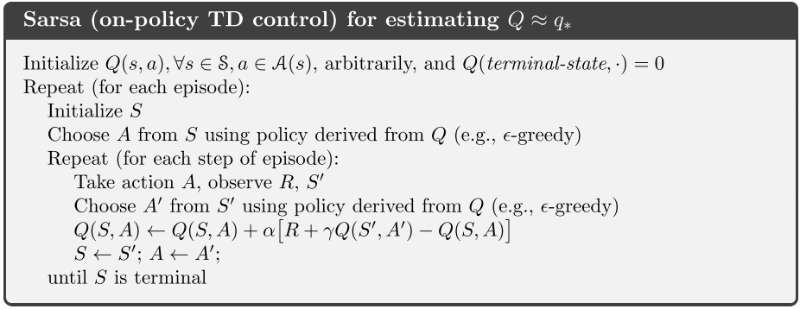
\includegraphics[width=0.7\columnwidth]{figures/sarsa-alg.jpg}
  \end{figure}

  \begin{figure}[t]
  	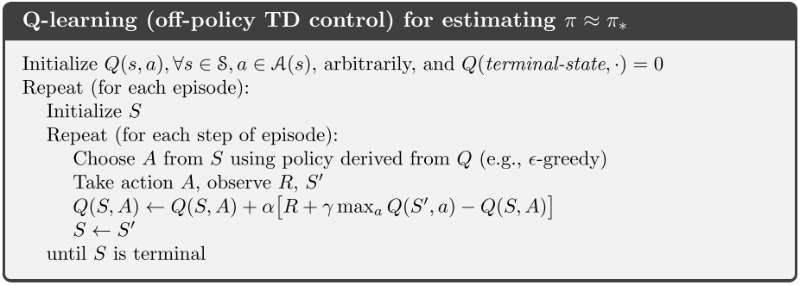
\includegraphics[width=0.7\columnwidth]{figures/q-learning-alg.jpg}
  \end{figure}
\end{frame}

\begin{frame}{Difference}
  \begin{itemize}
  	\item Exploration
  		\begin{itemize}
  			\item Sarsa: on-policy
  			\item Q-learning: off-policy
  		\end{itemize}
  	\item Update Rule
	  	\begin{itemize}
	  		\item Sarsa
	  		\begin{equation}\nonumber
	  		\begin{aligned}
	  		& Choose~ A'~ from~ S'~ using~policy~derived~from~Q~(e.g. \epsilon-greedy) \\
	  		& Q(S,A) \leftarrow Q(S,A) + \alpha[r + \gamma Q(S', A') - Q(S,A)]
	  		\end{aligned}
	  		\end{equation}
	  		\item Q-learning
	  		\begin{equation}\nonumber
	  		Q(S,A) \leftarrow Q(S,A) + \alpha[r + \gamma \max_a Q(S', a) - Q(S,A)]
	  		\end{equation}
	  	\end{itemize}
  \end{itemize}
\end{frame}




\section{Issues in Q-learning}

\subsection{Overestimation}
\begin{frame}{Overestimation}{Preliminaries}
	Recall that
	\begin{equation}
		Q(s,a) \longleftarrow r^a_s + \gamma~\red{\max}_{\ha} Q(s', \ha)
	\end{equation}
	Repeated application of this update equation eventually yields Q-values that give rise to \blue{a policy which maximizes the expected cumulative discounted reward}\footnote{C. J. C. H.Watkins, Learning from Delayed Rewards. PhD thesis, King’s College, Cambridge, England, 1989.} in the look-up table case.
	
	The \red{$\max$} operation may cause some problems under the approximation scenario.
\end{frame}

\begin{frame}{Overestimation}
	Assume $Q^{approx}(\cdot)$ representing implicit target values $Q^{target}$, corrupted by a noise term $Y$ such that
	\begin{equation}\nonumber
		\qa(s',\ha) = \qt(s', \ha) + Y_{s'}^{\ha}
	\end{equation}
	
	\begin{equation}
	\begin{aligned}
		Z_s &\overset{def}{=} r_s^a + \gamma~ \max_{\ha} \qa(s', \ha) - \left( r_s^a + \gamma~  \max_{\ha} \qt(s', \ha)\right) \\
		& = \gamma~ \left( \max_{\ha} \qa(s', \ha) - \max_{\ha} \qt(s', \ha)\right)
	\end{aligned}
	\end{equation}
	
	The key observation is
	\begin{equation}\nonumber
		E[Y_{s'}^{\ha}] = 0, ~ \forall \ha ~ \overset{often}{\Longrightarrow} E[Z_s] > 0 ~.
	\end{equation}
\end{frame}

\begin{frame}{Expectation of $Z$}
	\begin{Lemma}
		Let $n$ denote the number of actions applicable at state $s'$. If all $n$ actions share the same target Q-value, i.e., $\exists q: \forall \ha: q=\qt(s', \ha)$, then the average overestimation $E[Z_s]$ is $\gamma c$ with $c \overset{def}{=} \epsilon \frac{n-1}{n+1}$.
	\end{Lemma}

	The proof can be referred to the paper\footnote{\tiny{Thrun S, Schwartz A. Issues in using function approximation for reinforcement learning[C] Proceedings of the 1993 Connectionist Models Summer School Hillsdale, NJ. Lawrence Erlbaum. 1993.}}.
	\begin{Corollary}
		$0 \leq E[Z_s] \leq \gamma c$ with $c = \epsilon \frac{n-1}{n+1}$.
	\end{Corollary}
\end{frame}


\begin{frame}{Bounds for Expected Failure of Q-learning}{Simple Assumptions}
	\begin{itemize}
		\item There is a set of goal states;
		\item Positive reward $r_{goal}$ is only recieved upon entering a goal state;
		\item $r_{goal} = 1$;
		\item The state transition function is deterministic.
	\end{itemize}

	One \textit{necessary} condition for the success of Q-learning is that the sequence of Q-values $Q(s_i, a_i)$ is monotonically increasing in $i$:
	\begin{equation}
		Q(s_i, a_i) \leq Q(s_{i+1}, a_{i+1}), for~all~ i \in \{0, \ldots, L-1\}
	\end{equation}
\end{frame}

\begin{frame}{Bounds for Expected Failure of Q-learning}{Simple Assumptions}
Case 1: the learner \textit{always} overestimates Q-values by $\gamma c$.
\begin{Theorem}
	If there is maximal, repeated overestimation of magnitude $\gamma c$ along an optimal path, Q-learning is expected to fail to learn an optimal policy if $\gamma > \frac{1}{1+c}$.
\end{Theorem}
\end{frame}

\begin{frame}
Case 2: Assume that Q-learning managed to learn the \textit{last} L-1 Q-values of this optimal path correctly.

\begin{itemize}
	\item Q-values are given by iteratively discounting the final reward with the \textit{distance} to the goal state, i.e., \red{$Q(s_{L-i}, a_{L-i}) = \gamma^i$} for $i \in \{1,\ldots,L-1\}$.
	\item \textit{Correct} Q-value $Q^{correct}(s_0, a_0)$ is $\gamma^L$.
	
	\item In order to maintain monotonicity of Q, we need to make sure that
	\begin{equation}
	\gamma^{L-1} - \gamma^L \geq \gamma c ~.
	\end{equation}
\end{itemize}
\begin{theorem}
	Under the conditions above, Q-learning is expected to fail if
	\begin{equation}
		\gamma^{L-1} - \gamma^L < \gamma c ~.
	\end{equation}
\end{theorem}
\end{frame}

\begin{frame}
	\begin{theorem}
		Under the conditions above, Q-learning is expected to fail if
		\begin{equation}
			\epsilon > \frac{n+1}{n-1}\cdot \frac{(L-2)^{L-2}}{(L-1)^{L-1}} ~.
		\end{equation}
	\end{theorem}
\end{frame}

\subsection{Double Q-learning}

\begin{frame}{Double Q-learning}{Preliminaries}
	\begin{itemize}
		\item a set of random variables $X = \{X_i, \ldots, X_M\}$
			Our interest is that
			\begin{equation}\label{eq:objective}
				\max_i E[X_i] ~,
			\end{equation}
			which is in the Q-learning update rule.
		\item $S = \cup_{i=1}^M S_i$ where $S_i$ is the subset contains samples for the variable $X_i$ and each $s \in S_i$ is i.i.d.
		\item $E[X_i] = E[\mu_i] \approx \mu_i(S) \overset{def}{=}\frac{1}{|S_i|}\sum_{s\in S_i}s$ ~, where $\mu_i$ is an unbiased estimate for the value of $E[X_i]$.
		\item $f_i^{\mu}$ is PDF and $F_i^{\mu}$ is CDF of $X_i$.
	\end{itemize}
	\begin{equation}\nonumber
		\max_i E[X_i] = \max_i \int_{-\infty}^{\infty} x ~f_i^{\mu}(x)dx ~.
	\end{equation}
\end{frame}

\begin{frame}{Double Q-learning}{Single Estimator}
An obvious way to approximate the value in Eq.~(\ref{eq:objective}) is
	\begin{equation}
		\max_i E[X_i] = \max_i E[\mu_i] \approx \max_i \mu_i(S) ~.
	\end{equation}
	\begin{itemize}
		\item Assume the maximal estimator \red{$\max_i \mu_i(S)$} is distributed as PDF $f_{max}^{\mu}$.
		\item $f_{max}^{\mu} \neq f_i^{\mu}$ but $f_{max}^{\mu}$ is dependent on $f_i^{\mu}$.
		\pause
		\item CDF $F_{max}^{\mu}(x) \overset{def}{=} P(\max_i \mu_i \leq x) = \prod_{i=1}^M P(\mu_i \leq x) \overset{def}{=} \prod_{i=1}^M F_i^{\mu}(x) ~.$
	\end{itemize}
\end{frame}

\begin{frame}{Double Q-learning}{Biased Estimation of $E[X_i]$}
	\begin{itemize}
		\item The value $\max_i \mu_i(S)$ is an unbiased estimate for $E[\max_j \mu_j]$.
	\end{itemize}
	\begin{equation}\label{eq:single_est}
	\begin{aligned}
		E[\max_i \mu_i] &= \int_{-\infty}^{\infty} x ~f_{max}^{\mu}(x) \\
		&= \int_{-\infty}^{\infty}x\frac{d}{dx}\prod_{i=1}^M F_i^{\mu}(x)dx \\
		&= \sum_j^M \int_{-\infty}^{\infty}x ~f_j^{\mu}(s) \prod_{i\neq j}^M F_i^{\mu}(x)dx ~.
	\end{aligned}
	\end{equation}
	\begin{itemize}
		\item $\red{E}[\blue{\max}_i \mu_i]$ is not the same as $\blue{\max}_i \red{E}[X_i]$.
	\end{itemize}
\end{frame}

\begin{frame}{Double Q-learning}{Double Estimators}
	\begin{itemize}
		\item Two sets of estimators: $\mu^A={\mu_1^A,\ldots,\mu_M^A}$, $\mu^b={\mu_1^B,\ldots,\mu_M^B}$.
		\item Two subsets of samples: $S=S^A\cup S^B,~S^A \cap S^B = \emptyset$
		\item $\mu_i^A(S) \overset{def}{=}\frac{1}{|S^A_i|}\sum_{s\in S^A_i}s$, $\mu_i^B(S) \overset{def}{=}\frac{1}{|S^B_i|}\sum_{s\in S^B_i}s$.
	\end{itemize}

	\begin{itemize}
		\item Both $\mu_i^A$ and $\mu_i^B$ are unbiased if we assume proper split on the sample set $S$.
		\item $Max^A(S) \overset{def}{=} \{ j | \max_i \mu_i^A(S)\}$.
		\item Since $\mu_i^B(S)$ is an independent, unbiased set of estimators, we have $E[\mu_j^B(S)] = E[X_j]$ for all $j$ including $j \in Max^A$. We can pick $a^*$ such that $\mu_{a^*}^A \overset{def}{=} \max_i \mu_i^A(S)$. So that
		\begin{equation}
			\max_i E[X_i] = \max_i E[\mu_i^B] \approx \mu_{a^*}^B ~.
		\end{equation}
	\end{itemize}
\end{frame}

\begin{frame}{Double Q-learning}{Difference Between Single/Double Estimators}
	\begin{equation}
	\begin{aligned}
		P(j=a^*) &= \int_{-\infty}^{\infty} P(\mu_j^A = x) \prod_{i\neq j}^M P(\mu_j^A <x) dx \\
		&\overset{def}{=} \int_{-\infty}^{\infty} f_j^A(x) \prod_{i\neq j}^M F_i^A(x) dx 
	\end{aligned}
	\end{equation}
	
	\begin{equation}\label{eq:double_est}
		\sum_j^M \blue{P(j=a^*)} E[\mu_j^B] = \sum_j^M \red{E[\mu_j^B]} \int_{-\infty}^{\infty} f_j^A(x) \prod_{i\neq j}^M F_i^A(x) dx ~.
	\end{equation}
	
	Recall Eq.~(\ref{eq:single_est}) of single estimator that
	\begin{equation}\nonumber
	E[\max_i \mu_i] = \int_{-\infty}^{\infty} x ~f_{max}^{\mu}(x) = \sum_j^M \int_{-\infty}^{\infty} \red{x} ~f_j^{\mu}(s) \prod_{i\neq j}^M \blue{F_i^{\mu}(x)} dx ~.
	\end{equation}
\end{frame}


\begin{frame}{Double Q-learning}{Algorithm\footnote{\tiny{Hasselt H V. Double Q-learning[C] Advances in Neural Information Processing Systems. 2010: 2613-2621.}}\footnote{\tiny{Van Hasselt H, Guez A, Silver D. Deep Reinforcement Learning with Double Q-Learning[C] AAAI. 2016: 2094-2100.}\\}}
	\begin{figure}[t]
		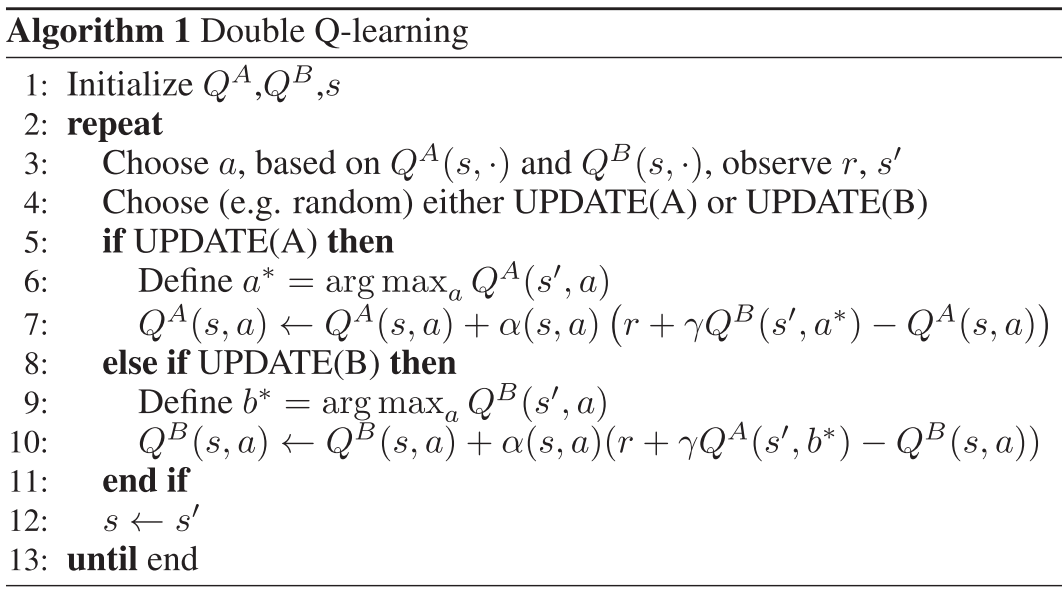
\includegraphics[width=0.7\columnwidth]{figures/double-q-learning-alg.jpg}
	\end{figure}
\end{frame}

\begin{frame}{Double Q-learning}{Performance}
\begin{figure}[t]
	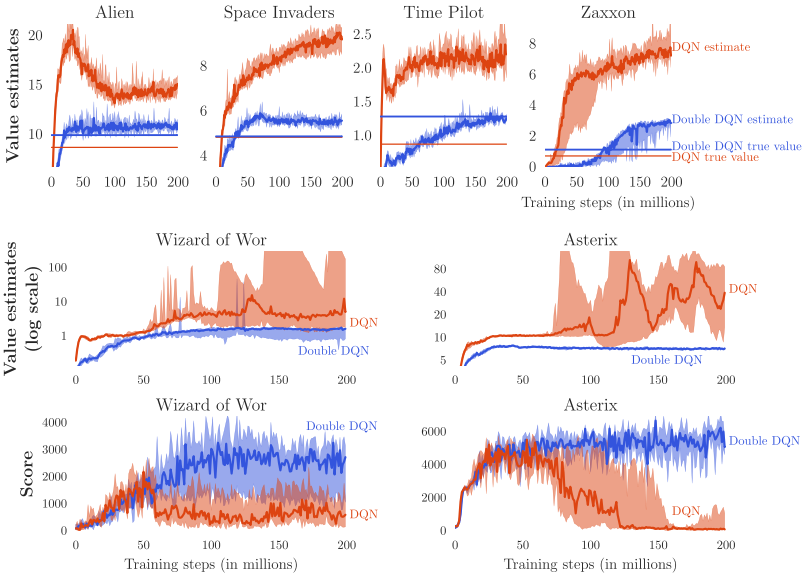
\includegraphics[width=0.7\columnwidth]{figures/ddqn-performance.jpg}
\end{figure}
\end{frame}


\subsection{Averaged Q-learning}

\begin{frame}{Averaged Deep Q-Network}
	\begin{itemize}
		\item Double Q-learning aims to correct the \textit{overestimation} of natural Q-learning.
		\item Averaged DQN focus on variance reduction and stabilization.
	\end{itemize}
\end{frame}

\begin{frame}{Averaged Deep Q-Network}{Revision of DQN\footnote{\tiny{Mnih V, Kavukcuoglu K, Silver D, et al. Human-level control through deep reinforcement learning[J]. Nature, 2015, 518(7540): 529-533.}}}
	\begin{figure}[t]
		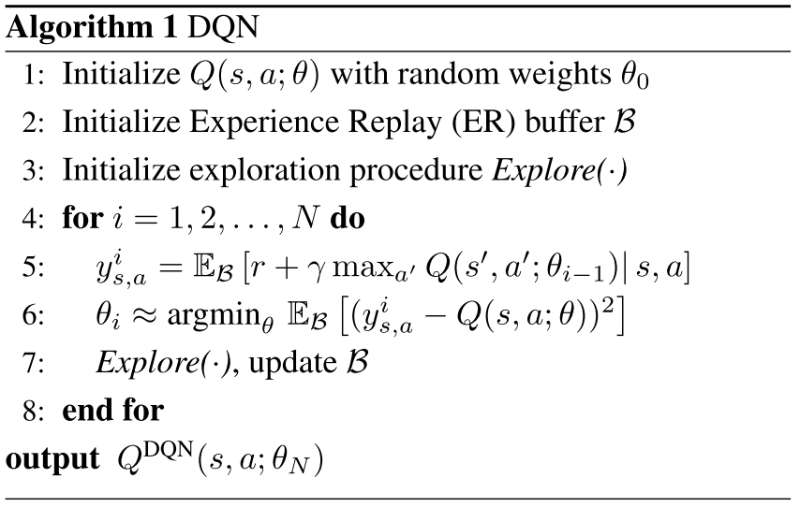
\includegraphics[width=0.7\columnwidth]{figures/dqn-alg.jpg}
	\end{figure}
\end{frame}


\begin{frame}{Averaged Deep Q-Network}{Algorithm\footnote{\tiny{Anschel O, Baram N, Shimkin N. Averaged-DQN: Variance Reduction and Stabilization for Deep Reinforcement Learning[C] International Conference on Machine Learning. 2017: 176-185.}}}
\begin{figure}[t]
	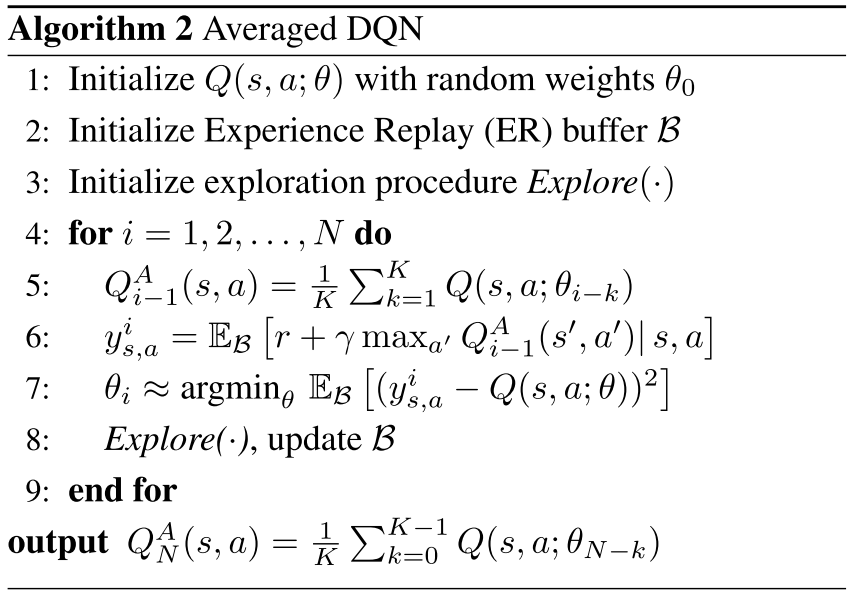
\includegraphics[width=0.7\columnwidth]{figures/adqn-alg.jpg}
\end{figure}
\end{frame}


\begin{frame}{Averaged Deep Q-Network}{Performance}
\begin{figure}[t]
	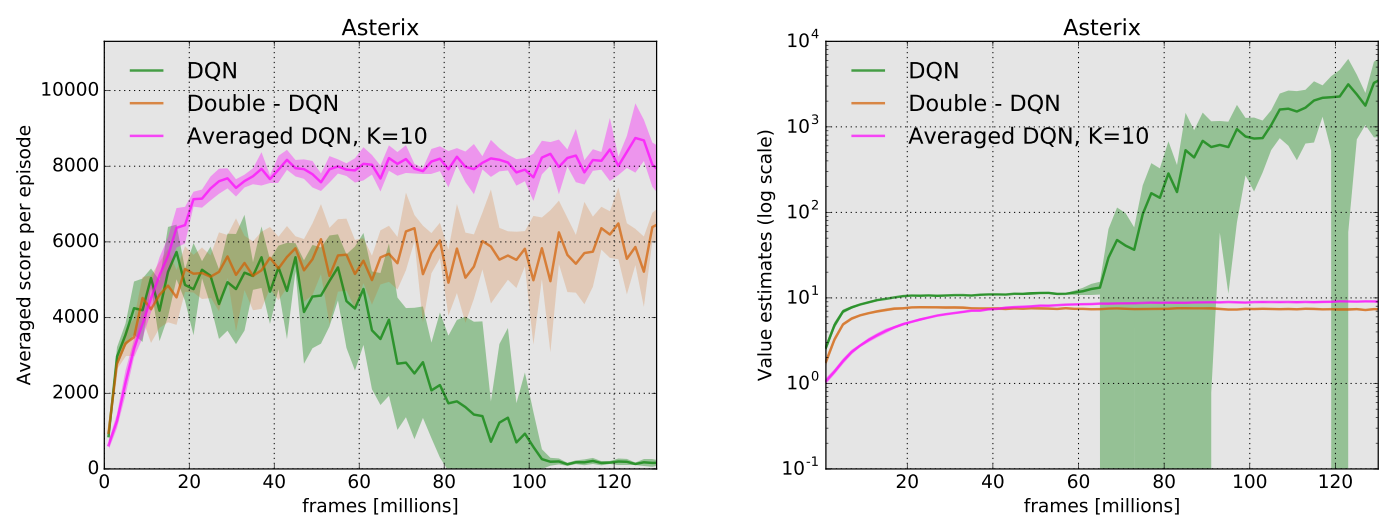
\includegraphics[width=0.88\columnwidth]{figures/adqn-performance.jpg}
\end{figure}
\end{frame}

\begin{frame}{Averaged Deep Q-Network}{Error Analysis}
Let $Q(s,a; \theta_i)$ be the value function of DQN at iteration $i$,
\begin{equation}
\begin{aligned}
	\Delta_i &= \qi - Q^*(s,a) \\
	&= \underbrace{\qi - y_{s,a}^i}_{\text{Target Apprixmation Error}} + \underbrace{y_{s,a}^i - \hat{y}_{s,a}^i}_{\text{Overestimation Error}} \\
	&~~~~ + \underbrace{ \hat{y}_{s,a}^i - Q^*(s,a)}_{Optimality Difference} ~.
\end{aligned}
\end{equation}

Here $y_{s,a}^i$ is the \textit{DQN target}, and $\hat{y}_{s,a}^i$ is the \textit{true target}, such that
\begin{equation}
\begin{aligned}
	y_{s,a}^i &= E_{\mathcal{B}} \left[ r + \gamma \max_{a'} Q(s', a'; \theta_i{i-1}) | s,a \right] ~,\\
	\hat{y}_{s,a}^i &= E_{\mathcal{B}} \left[ r + \gamma \max_{a'} ( \hat{y}^{i-1}_{s',a'} ) | s,a \right] ~.
\end{aligned}
\end{equation}
\end{frame}

\begin{frame}{Averaged Deep Q-Network}{Background and Related Work}
Define $Z_{s,a}^i$ as TAE (Target Approximation Error) and $R_{s,a}^i$ as overestimation error.
	\begin{equation}
	\begin{aligned}
		Z_{s,a}^i &= Q(s,a; \theta_i) - y_{s,a}^i ~,\\
		R_{s,a}^i &= y_{s,a}^i - \hat{y}_{s,a}^i ~.
	\end{aligned}
	\end{equation}
	
In Thrun \& Schwartz (1993), $Z_{s,a}^i$ is considered as a random variable uniformly distributed error in $[-\epsilon, \epsilon]$ and
\begin{equation}
	E_{\red{z}}[R_{s,a}^i] = \gamma E_{\red{z}}[\max_{a'}[Z_{s',a'}^{i-1}]] = \gamma \epsilon \frac{n-1}{n+1} ~.
\end{equation}

In Double Q-learning paper, the author replaces \textit{positive} bias with a \textit{negative} one.
\end{frame}


\begin{frame}{Averaged Deep Q-Network}{TAE Variance Reduction}
Assume that
\begin{equation}
\begin{aligned}
	&E[Z_{s,a}^i] = 0,~ Var[Z_{s,a}^i] = \sigma_s^2, \\
	&\text{for}~ i \neq j, Cov[Z_{s,a}^i, Z_{s',a'}^j] = 0.
\end{aligned}
\end{equation}
We consider a fixed policy for updating the target values, and conveniently consider a zero reward $r=0$ everywhere since it has no effect on variance calculations.
\end{frame}


\begin{frame}{Averaged Deep Q-Network}{TAE Variance Reduction (cont.)}
Consider M-state unidirectional MDP as
\begin{figure}[t]
	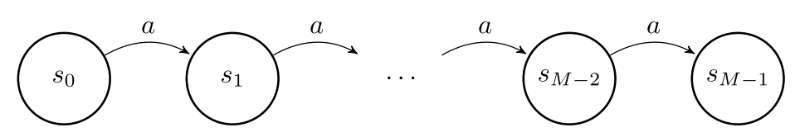
\includegraphics[width=0.6\columnwidth]{figures/m-mdp.jpg}
\end{figure}

\begin{equation}
\begin{aligned}
	& Q^{DQN}(s_0, a; \theta_i) = Z_{s_0,a}^i + y_{s_0,a}^i \\
	& ~~~ = Z_{s_0,a}^i + \gamma Q(s_1, a; \theta_{i-1}) \\
	& ~~~ = Z_{s_0,a}^i + \gamma [Z_{s_1,a}^{i-1} + y_{s_1,a}^{i-1}] = \ldots = \\
	& ~~~ = Z_{s_0,a}^i + \gamma Z_{s_1,a}^{i-1} + \ldots + \gamma^{M-1} Z_{s_{M-1},a}^{i-(M-1)}
\end{aligned}
\end{equation}
Since $\text{for}~ i \neq j, Cov[Z_{s,a}^i, Z_{s',a'}^j] = 0$, we have
\begin{equation}
	Var[Q^{DQN}(s_0, a; \theta_i)] = \sum_{m=0}^{M-1}\gamma^{2m}\sigma_{s_m}^2 ~.
\end{equation}
\end{frame}

\begin{frame}{Averaged Deep Q-Network}{TAE Variance Reduction (cont.)}
For Averaged DQN,
\begin{equation}
Q_i = Z_i + \gamma P\frac{1}{K} \sum_{k=1}^{K} Q_{i-k} ~,
\end{equation}
where $P \in \mathbb{R}_+^{S\times S}$ is the transition probabilities matrix for the given policy.
Recall that $Z_{s,a}^i = Q(s,a; \theta_i) - y_{s,a}^i $.
\end{frame}


\begin{frame}{Averaged Deep Q-Network}{Ensemble DQN}
\begin{figure}[t]
	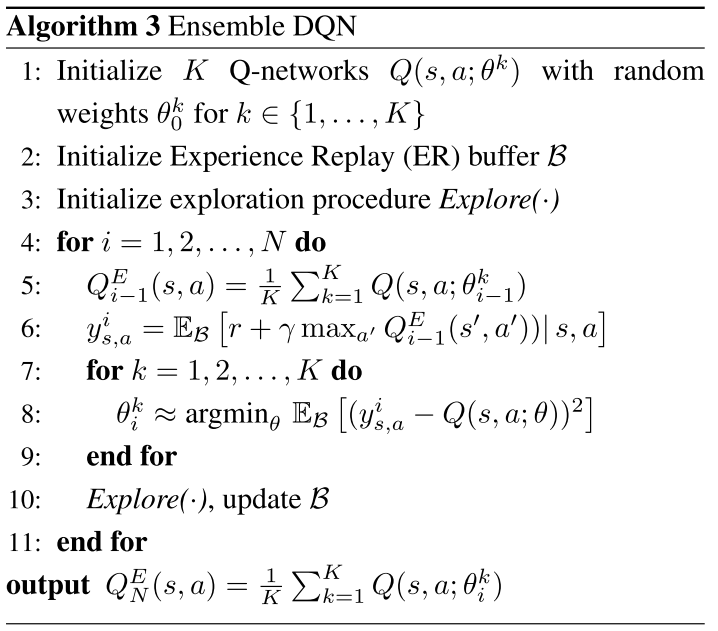
\includegraphics[width=0.6\columnwidth]{figures/edqn-alg.jpg}
\end{figure}
\end{frame}

\begin{frame}{Averaged Deep Q-Network}{Ensemble DQN Variance}
For $i > M$,
\begin{equation}
\begin{aligned}
	Q_i^E(s_0, a) &= \sum_{m=0}^{M-1}\gamma^m \frac{1}{K} \sum_{k=1}^{K} Z_{s_m,a}^{k, i-m} \\
	Var[Q_i^E(s_0, a)] &= \sum_{m=0}^{M-1} \frac{1}{K} \gamma^{2m} \sigma_{s_m}^2 \\
	&= \frac{1}{K} Var[Q^{DQN}(s_0, a; \theta_i)]
\end{aligned}
\end{equation}
\end{frame}


\begin{frame}{Averaged Deep Q-Network}{Averaged DQN Variance}
For $i > KM$,
\begin{equation}
	Var[Q_i^A(s_0, a)] = \sum_{m=0}^{M-1} D_{K,m} \gamma^{2m} \sigma_{s_m}^2 ~,
\end{equation}
where $D_{K,m} = \frac{1}{N} \sum_{n=0}^{N-1} | U_n/K |^{2(m+1)}$ and $U = (U_n)_{n=0}^{N-1}$ denoting a Discrete Fourier Transform of a rectangle pulse.

Furthermore, $D_{K,m} < \frac{1}{K}$ and
\begin{equation}
\begin{aligned}
	Var[Q_i^A(s_0, a)] &< Var[Q_i^E(s_0, a)] \\
	&= \frac{1}{K} Var[Q^{DQN}(s_0, a; \theta_i)] ~.
\end{aligned}
\end{equation}
\end{frame}



\section{Deep Q-network}

\subsection{Nature DQN}
\subsection{Several Imrovements}

\begin{frame}{Q-networks}
	Represent value function by \red{Q-network} with weights $w$
	\begin{equation}
		Q(s,a; w) \approx Q^*(s,a) ~.
	\end{equation}
	
	\begin{figure}[t]
		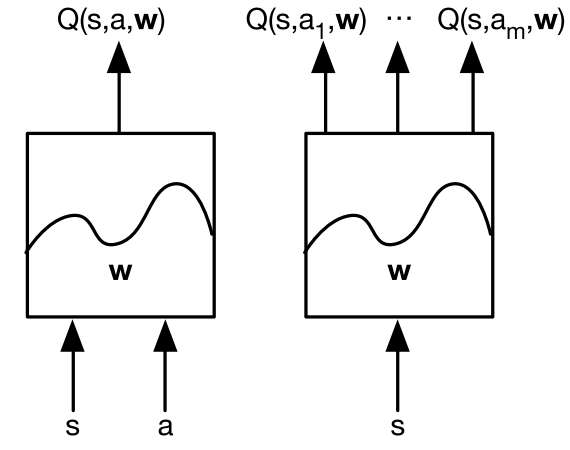
\includegraphics[width=0.4\columnwidth]{figures/q-network.jpg}
	\end{figure}
\end{frame}

\begin{frame}{Deep Q-network}
Refer to D. Silver's slides P31 - P45.
\end{frame}

\begin{frame}{Duelling network}
	\begin{figure}
		\centering
		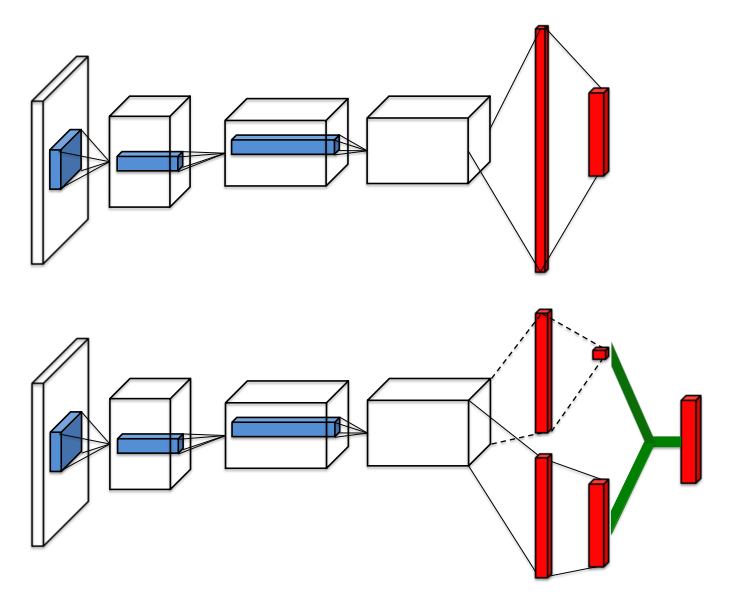
\includegraphics[width=0.65\linewidth]{figures/duel-network}
		\caption{Duelling network: split Q-network into two channels}
		\label{fig:duel-network}
	\end{figure}
\end{frame}


\section{Convergence of Tabular TD}
\subsection{Sarsa}

\begin{frame}{Convergence of Sarsa(0)}{Convergence of Random Iterative Process}
\begin{lemma}
	A random iterative process
	\begin{equation}\label{eq:random-iterarive-process}
		\Delta_{t+1}(x) = (1-\alpha_t(x)) \Delta_{t}(x) + \alpha_t(x)F_t(x), ~x\in X, ~t=0,1,2,\ldots
	\end{equation}
	converges to zero w.p.1 if the following properties hold:
	\small{
	\begin{itemize}
		\item 1. the set of possible states $X$ is finite.
		\item 2. $0 \leq \alpha_t(x) \leq 1, \sum_t \alpha_t(x) = \infty, \sum_t \alpha_t^2(x) < \infty ~ w.p.1$, where the probability is over the learning rates $\alpha_t$.
		\item 3. $\| E[F_t(\cdot) | P_t] \|_W \leq \kappa \| \Delta_{t} \|_W + c_t$, where $\kappa \in [0,1)$ and $c_t$ converges to zero w.p.1.
		\item 4. $Var[F_t(x)] \leq K(1 + \| \Delta_t \|_W)^2$, where K is some constant.
	\end{itemize}
	}
	\tiny{Here $P_t$ is an increasing sequence of $\sigma$-fields that includes the past of the process. In particular we assume that $\alpha_t, \Delta_t, F_{t-1} \in P_t$.
	The notation $\|\cdot\|_W$ refers to some (fixed) weighted maximum norm.}
\end{lemma}
\end{frame}


\begin{frame}{Convergence of Sarsa(0)}
	\begin{theorem}
		In finite state-action MDPs, the $Q_t$ values computed by the Sarsa(0) rule
		\small{
		\begin{equation}\nonumber
		\begin{aligned}
			Q_{t+1}(s_t, a_t) &= Q_t(s_t, a_t) + \alpha_t(s_t, a_t)[r_t + \gamma Q_t(s_{t+1}, a_{t+1}) - Q_t(s_t, a_t)] \\
			&= (1-\alpha(s_t, a_t)) Q_t(s_t, a_t) + \alpha_t(s_t, a_t)[r_t + \gamma Q_t(s_{t+1}, a_{t+1})] ~.
		\end{aligned}
		\end{equation}
		}
		converges to $Q^*$ and the learning policy $\pi_t$ converges to an optimal policy $\pi^*$ if the learning policy is GLIE with these additional conditions are satisfied
		\begin{itemize}
			\item 1. The Q values are stored in a lookup table.
			\item 2. The learning rates satisfy $0 \leq \alpha_t(s_t, a_t) \leq 1, ~\sum_t \alpha_t(s_t, a_t) = \infty, \sum_t \alpha_t^2(s_t, a_t) < \infty$ and $\alpha_t(s_t, a_t) = 0$ unless $(s, a) = (s_t, a_t)$.
			\item 3. $Var[r(s,a)] < \infty$ .
		\end{itemize}
	\end{theorem}
\end{frame}


\begin{frame}{Convergence of Sarsa(0)}
\begin{itemize}
	\item $x \overset{def}{=} (s_t, a_t)$.
	\item $\Delta_{t} \overset{def}{=} Q_t(s, a) - Q^*(s,a)$.
\end{itemize}
So we get
\begin{equation}
\begin{aligned}
	\Delta_{t+1}(s_t, a_t) &= Q_{t+1}(s_t, a_t) - Q^*(s,a) \\
	&= (1-\alpha(s_t, a_t)) \Delta_{t}(s_t, a_t) + \alpha_t(s_t, a_t)F_t(s_t, a_t).
\end{aligned}
\end{equation}
where
\begin{equation}
\begin{aligned}
	F_t(s_t, a_t) &= r_t + \gamma \max_{a'} Q_t(s_{t+1}, a') - Q^*(s_t, a_t) \\
	& + \gamma \left[ Q_t(s_{t+1}, a_{t+1}) - \max_{a'} Q_t(s_{t+1}, a') \right] \\
	& \overset{def}{=} \blue{r_t + \gamma \max_{a'} Q_t(s_{t+1}, a') - Q^*(s_t, a_t)} + C_t(Q) \\
	& \overset{def}{=} \blue{F_t^Q(s_t,a_t)} + C_t(s_t, a_t)
\end{aligned}
\end{equation}
\end{frame}


\subsection{Q-learning (TBE)}

\end{document}


